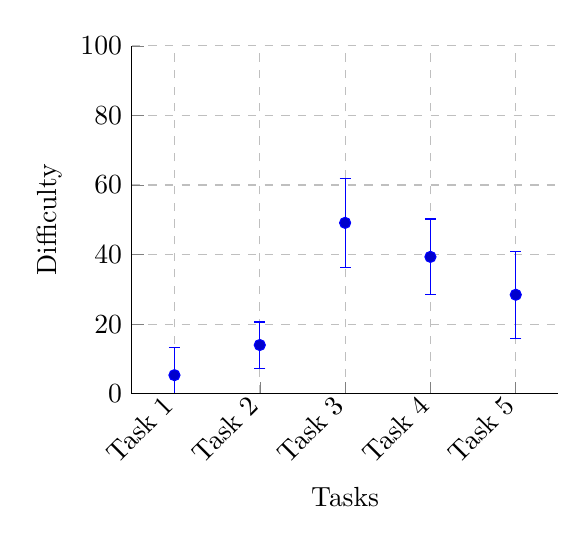
\begin{tikzpicture}[scale=1.0],
\centering
\begin{axis}[
height=6cm,
width=7cm,
  xlabel={Tasks},
  ylabel={Difficulty}, 
  ymax=100,
  ymin=0,
  xmin=0.5,
  xmax=5.5,
  axis y line*=left,
  axis x line*=bottom,
  xticklabels={Task 1,Task 2,Task 3,Task 4,Task 5},
  xtick={1,...,5},
  ytick={0,20,...,200},
  ymajorgrids=true,
  xmajorgrids=true,
  grid style=dashed,
  x tick label style={rotate=45,anchor=east}]
\addplot+[only marks][error bars/.cd,y dir=both, y explicit]
coordinates {
(1,5.3333) +- (8.0248,8.0248)
(2,14) +- (6.629,6.629)
(3,49.111) +- (12.721,12.721)
(4,39.333) +- (10.892,10.892)
(5,28.444) +- (12.445,12.445)
};
\addplot[dashed] coordinates {(0,0) (5.5,0)};
\end{axis}
\end{tikzpicture}%